% --------------------------------------------------------------------------- %
% Beamer slides adapted from the poster poster/covid_mortality.tex             %
% COVID-19 disrupted patterns of cause-specific mortality in Switzerland       %
% Compile with: pdflatex (twice) or latexmk -pdf                               %
% --------------------------------------------------------------------------- %
\documentclass[aspectratio=169,10pt]{beamer}

\usetheme{default}
\usecolortheme{default}
\setbeamertemplate{navigation symbols}{}
\setbeamertemplate{caption}[numbered]
\setbeamertemplate{itemize items}[circle]
\setbeamertemplate{frametitle}[default][left]

\usepackage[scaled]{helvet}
\renewcommand{\familydefault}{\sfdefault}

\usepackage[T1]{fontenc}
\usepackage[utf8]{inputenc}
\usepackage{graphicx}
\usepackage{amsmath}
\usepackage{booktabs}
\usepackage{array}

%%% Colors taken from the poster %%%%%%%%%%%%%%%%%%%%%%%%%%%%%%%%%%%%%%%%%%%%%%
\definecolor{headerfontcol}{RGB}{190,0,0}   % poster title red
\definecolor{bordercol}{RGB}{105,105,105}

\setbeamercolor{frametitle}{fg=headerfontcol,bg=white}
\setbeamercolor{title}{fg=headerfontcol}
\setbeamercolor{structure}{fg=headerfontcol}
\setbeamercolor{footline}{fg=bordercol}
\setbeamerfont{frametitle}{series=\bfseries}
\setbeamerfont{title}{series=\bfseries}

%%% Slide number in the footer %%%%%%%%%%%%%%%%%%%%%%%%%%%%%%%%%%%%%%%%%%%%%%%%
\setbeamertemplate{footline}{%
  \hfill\usebeamercolor[fg]{footline}%
  \scriptsize\insertframenumber/\inserttotalframenumber\hspace*{2ex}\vspace*{1ex}%
}

%%% Figures live next to the poster; keep a local copy path as a fallback %%%%%%
\graphicspath{{./}{images/}{../poster/}{../poster/images/}}

%%% Compact itemize, mirroring \compresslist from the poster %%%%%%%%%%%%%%%%%%%
\newcommand{\compresslist}{%
  \setlength{\itemsep}{2pt}%
  \setlength{\parskip}{0pt}%
  \setlength{\parsep}{0pt}%
}

%%% Small caption text under figures %%%%%%%%%%%%%%%%%%%%%%%%%%%%%%%%%%%%%%%%%%
\newcommand{\figcaption}[1]{{\tiny #1}}

%%%%%%%%%%%%%%%%%%%%%%%%%%%%%%%%%%%%%%%%%%%%%%%%%%%%%%%%%%%%%%%%%%%%%%%%%%%%%%%
\title{\large COVID-19 disrupted patterns of cause-specific mortality in Switzerland}
\author{\small Anthony Hauser\inst{1}\thanks{anthony.hauser@unisante.ch} \and
  Moritz Wagner\inst{2} \and Anna Fesser\inst{2} \and Karim Abawi\inst{3} \and
  Anne Laube\inst{2} \and Garyfallos Konstantinoudis\inst{4} \and Julien Riou\inst{1}}
\institute{\scriptsize
  \inst{1} Department of Epidemiology and Health Systems, Unisant\'e, Center for Primary Care
  and Public Health and University of Lausanne, Lausanne, Switzerland \\
  \inst{2} Federal Statistical Office, Neuch\^atel, Switzerland \\
  \inst{3} Federal Office of Public Health, Communicable Diseases Division, Bern, Switzerland \\
  \inst{4} Grantham Institute for Climate Change and the Environment, Imperial College London, UK}
\date{\small\today}

%%%%%%%%%%%%%%%%%%%%%%%%%%%%%%%%%%%%%%%%%%%%%%%%%%%%%%%%%%%%%%%%%%%%%%%%%%%%%%%
\begin{document}

\begin{frame}[plain]
  \titlepage
\end{frame}

%%% Background %%%%%%%%%%%%%%%%%%%%%%%%%%%%%%%%%%%%%%%%%%%%%%%%%%%%%%%%%%%%%%%%
\begin{frame}{Background}
  \begin{itemize}\compresslist
    \item The COVID-19 pandemic reshaped mortality through:
      \begin{itemize}\compresslist
        \item direct deaths from SARS-CoV-2,
        \item associated deaths from other causes (e.g., cardiovascular diseases)
              triggered by infection,
        \item mortality displacement across time and causes,
        \item indirect effects of control measures and behavioural changes
              (e.g., fewer respiratory infections, healthcare disruptions).
      \end{itemize}
    \item These disruptions occur \textbf{simultaneously across multiple causes},
          limiting the interpretability of all-cause and single-cause excess mortality.
    \item A \textbf{multivariate approach} is necessary to capture cross-cause
          dependencies and facilitate the interpretation of these disruptions.
  \end{itemize}
\end{frame}

%%% Objectives %%%%%%%%%%%%%%%%%%%%%%%%%%%%%%%%%%%%%%%%%%%%%%%%%%%%%%%%%%%%%%%%
\begin{frame}{Objectives}
  \begin{enumerate}\compresslist
    \item Implement a \textbf{Bayesian multivariate model} to estimate
          cause-specific excess mortality over time in Switzerland.
    \item Quantify \textbf{dependencies between mortality causes} before and
          during COVID-19.
    \item Identify the \textbf{mechanisms} driving mortality disruptions during
          the pandemic.
  \end{enumerate}
\end{frame}

%%% Data %%%%%%%%%%%%%%%%%%%%%%%%%%%%%%%%%%%%%%%%%%%%%%%%%%%%%%%%%%%%%%%%%%%%%%
\begin{frame}{Data}
  \begin{itemize}\compresslist
    \item \textbf{Cause-specific deaths}: $y_{irs}(t)$
      \begin{itemize}\compresslist
        \item aggregated by cause $i$, sex $s$, NUTS-2 region $r$, year and week $t$;
              by age group (0--17, 18--39, 40--64, 65--79, 80+); in 2011--2021,
        \item include immediate, underlying and contributing causes (ICD-10),
        \item grouped into 9 categories: cardiovascular (CVD), mental/neurological,
              respiratory, infectious diseases, cancer, external causes, suicide,
              COVID-19 and others.
      \end{itemize}
    \item \textbf{Population sizes}: $N_{rst}$ by age, sex and region;
          weekly estimates via linear interpolation.
  \end{itemize}
\end{frame}

%%% Model %%%%%%%%%%%%%%%%%%%%%%%%%%%%%%%%%%%%%%%%%%%%%%%%%%%%%%%%%%%%%%%%%%%%%
\begin{frame}{Model: expected mortality}
  For each age group, we fit the number of deaths $y_{irs}(t)$ due to underlying
  cause $i$ at year and week $t$, in region $r$ and sex $s$, between 2011 and 2019:
  \[
    y_{irs}(t) \sim \text{Poisson}\big(\mu_{irs}(t)\big)
  \]
  \[
    \log \mu_{irs}(t) = \alpha_i + \beta_{ir} + \gamma_{is}
      + f_{i}(t) + g_{i}(t) + \varepsilon_i(t) + \log N_{rst}
  \]
  where
  \begin{itemize}\compresslist
    \item $\alpha_i$, $\beta_{ir}$, $\gamma_{is}$: baseline mortality, effects of
          region and sex,
    \item $f_{i}(t)$, $g_{i}(t)$: long-term and seasonal trends (Gaussian processes),
    \item $\varepsilon_i(t)$: multivariate random effect,
          $\varepsilon(t) \sim \mathcal{N}(0,\Sigma)$.
  \end{itemize}
\end{frame}

\begin{frame}{Model: excess mortality}
  \[
    E_{irs}(t) := y_{irs}(t) - \tilde{y}_{irs}(t)
  \]
  where $\tilde{y}_{irs}(t)$ is the expected number of deaths, i.e., the posterior
  predictive distribution after removing $\varepsilon_i(t)$.
  \vfill
  \begin{itemize}\compresslist
    \item The covariance $\Sigma$ of $\varepsilon(t)$ captures the
          \textbf{cross-cause dependencies} of mortality.
    \item Excess mortality is obtained jointly for all causes, which allows
          correlations between cause-specific excesses to be quantified.
  \end{itemize}
\end{frame}

%%% Results 1 %%%%%%%%%%%%%%%%%%%%%%%%%%%%%%%%%%%%%%%%%%%%%%%%%%%%%%%%%%%%%%%%%
\begin{frame}{Temporal trends and cross-cause correlations}
  \begin{columns}[t]
    \begin{column}{0.42\linewidth}
      \begin{itemize}\compresslist
        \item The model captures seasonal and long-term trends of cause-specific
              mortality in 2011--2019 (Fig.~1, 80+).
        \item Expected mortality peaks between January and February for every cause.
        \item Shift in peak timing during COVID-19.
        \item Strong pairwise correlations in cause-specific excess mortality.
      \end{itemize}
    \end{column}
    \begin{column}{0.56\linewidth}
      \centering
      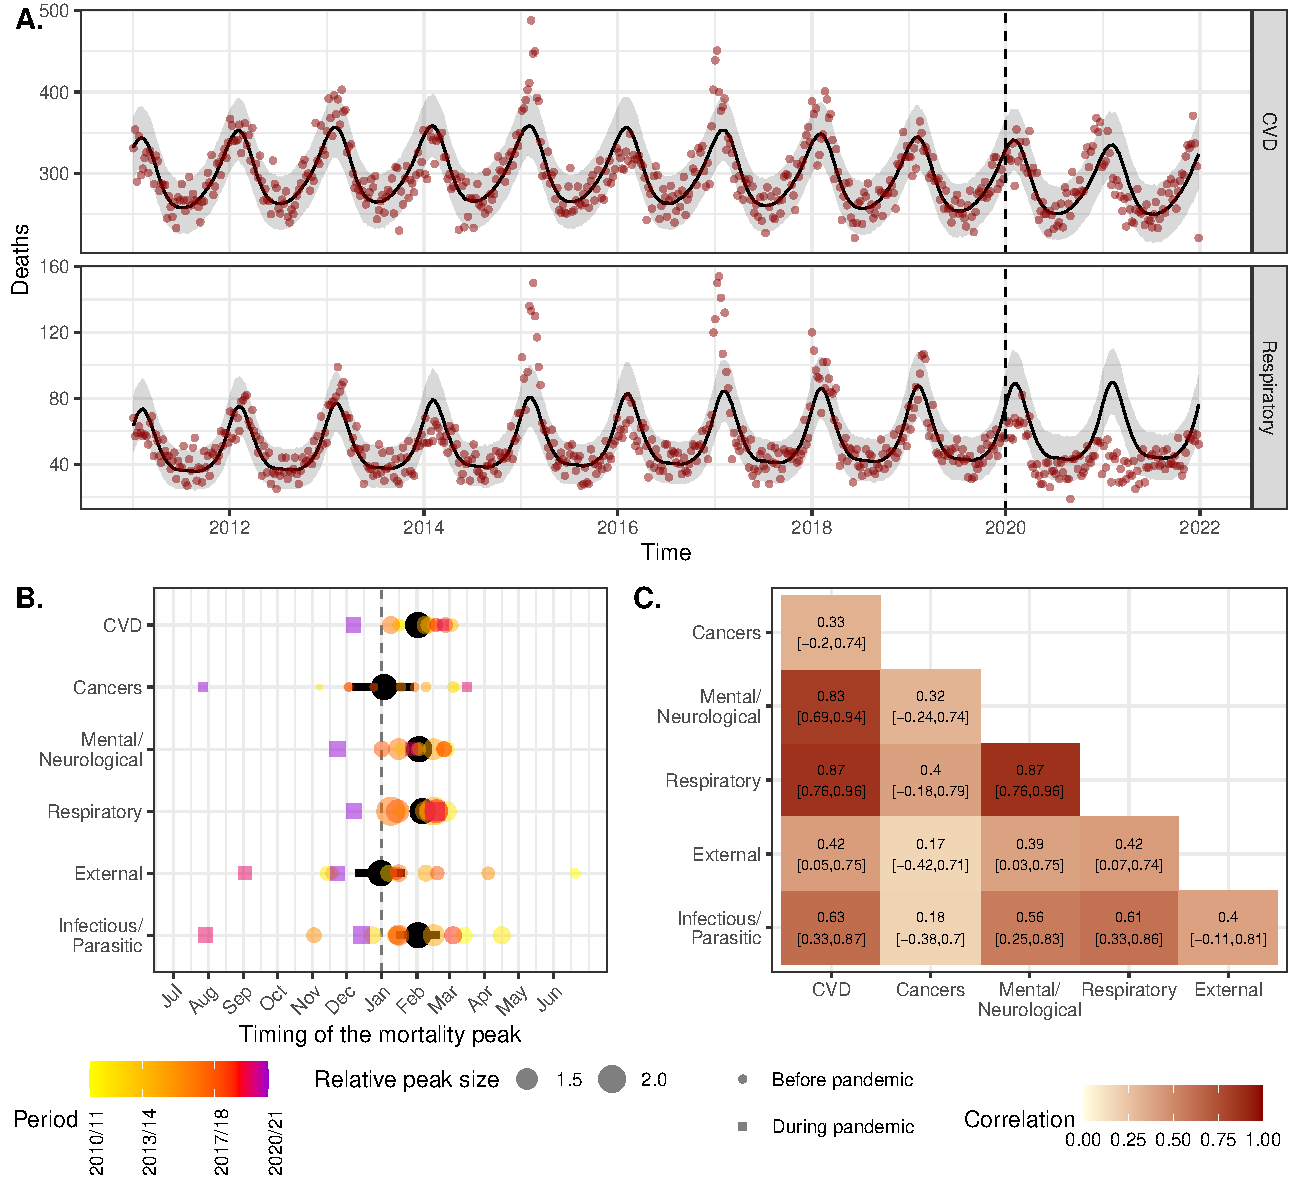
\includegraphics[width=\linewidth,height=0.72\textheight,keepaspectratio]{fig1_v4.pdf}\\[0.2em]
      \figcaption{\textbf{Figure 1. Model fit and cross-cause patterns for 80+.}
        A. Weekly deaths observed (red) and model estimates/predictions (black)
        with 95\% CrI (gray). B. Timing of mortality peaks; colored points:
        observed, black: posterior estimate with 95\% CrI.
        C. Cross-cause correlation of excess mortality.}
    \end{column}
  \end{columns}
\end{frame}

%%% Results 2 %%%%%%%%%%%%%%%%%%%%%%%%%%%%%%%%%%%%%%%%%%%%%%%%%%%%%%%%%%%%%%%%%
\begin{frame}{Impact of COVID-19 deaths on all-cause mortality}
  \begin{columns}[t]
    \begin{column}{0.55\linewidth}
      \centering
      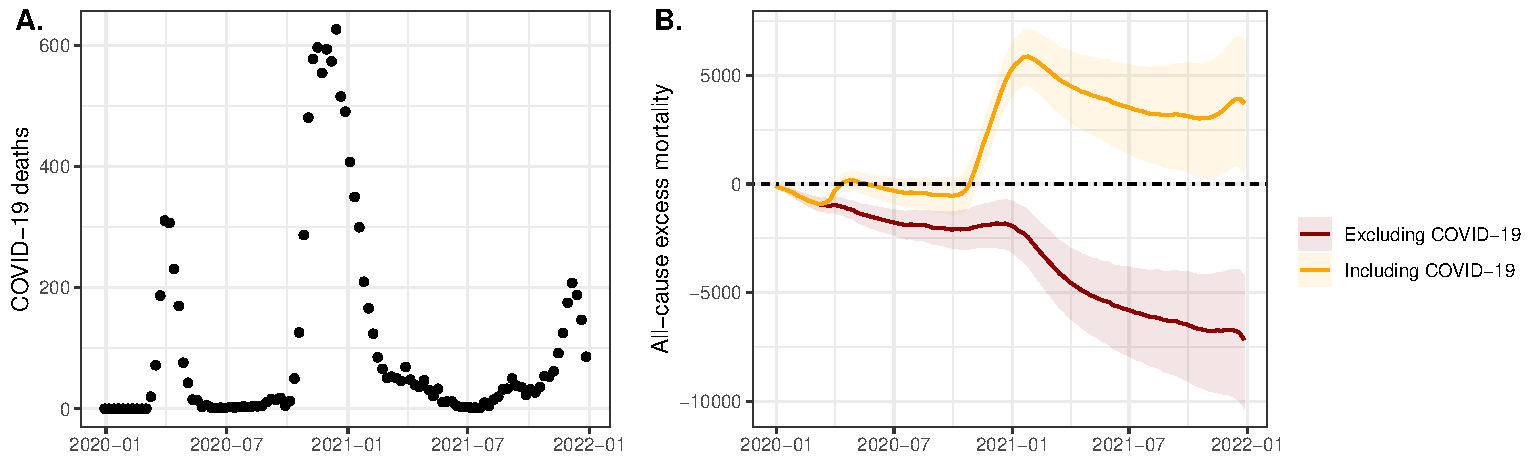
\includegraphics[width=\linewidth,height=0.7\textheight,keepaspectratio]{fig2_v2.pdf}\\[0.2em]
      \figcaption{\textbf{Figure 2.} A. Weekly COVID-19 deaths in 80+.
        B. Excess mortality with and without COVID-19 in 80+.}
    \end{column}
    \begin{column}{0.43\linewidth}
      \begin{itemize}\compresslist
        \item Sharp rise in cumulative excess mortality during major waves
              (Fig.~2, 80+).
        \item Subsequent weeks show a mortality deficit.
        \item When excluding COVID-19 deaths, mortality was \textbf{lower than
              expected} in 2020--21.
      \end{itemize}
    \end{column}
  \end{columns}
\end{frame}

%%% Results 3 %%%%%%%%%%%%%%%%%%%%%%%%%%%%%%%%%%%%%%%%%%%%%%%%%%%%%%%%%%%%%%%%%
\begin{frame}{Cause-specific mortality over time}
  \begin{columns}[t]
    \begin{column}{0.44\linewidth}
      \textbf{Cause-specific excess by phase}
      \begin{itemize}\compresslist
        \item CVD mortality excess concentrates during the COVID-19 waves,
              followed by deficits (Fig.~3, 80+).
        \item Strong mortality decrease for mental/neurological disorders
              ($-12\%$), especially during the Alpha wave ($-24\%$) in 80+.
        \item Cancer mortality deficit mainly during the Alpha wave in 80+.
        \item Respiratory (non-COVID) mortality consistently below expected across
              all ages, with larger deficits at older ages.
      \end{itemize}
    \end{column}
    \begin{column}{0.54\linewidth}
      \centering
      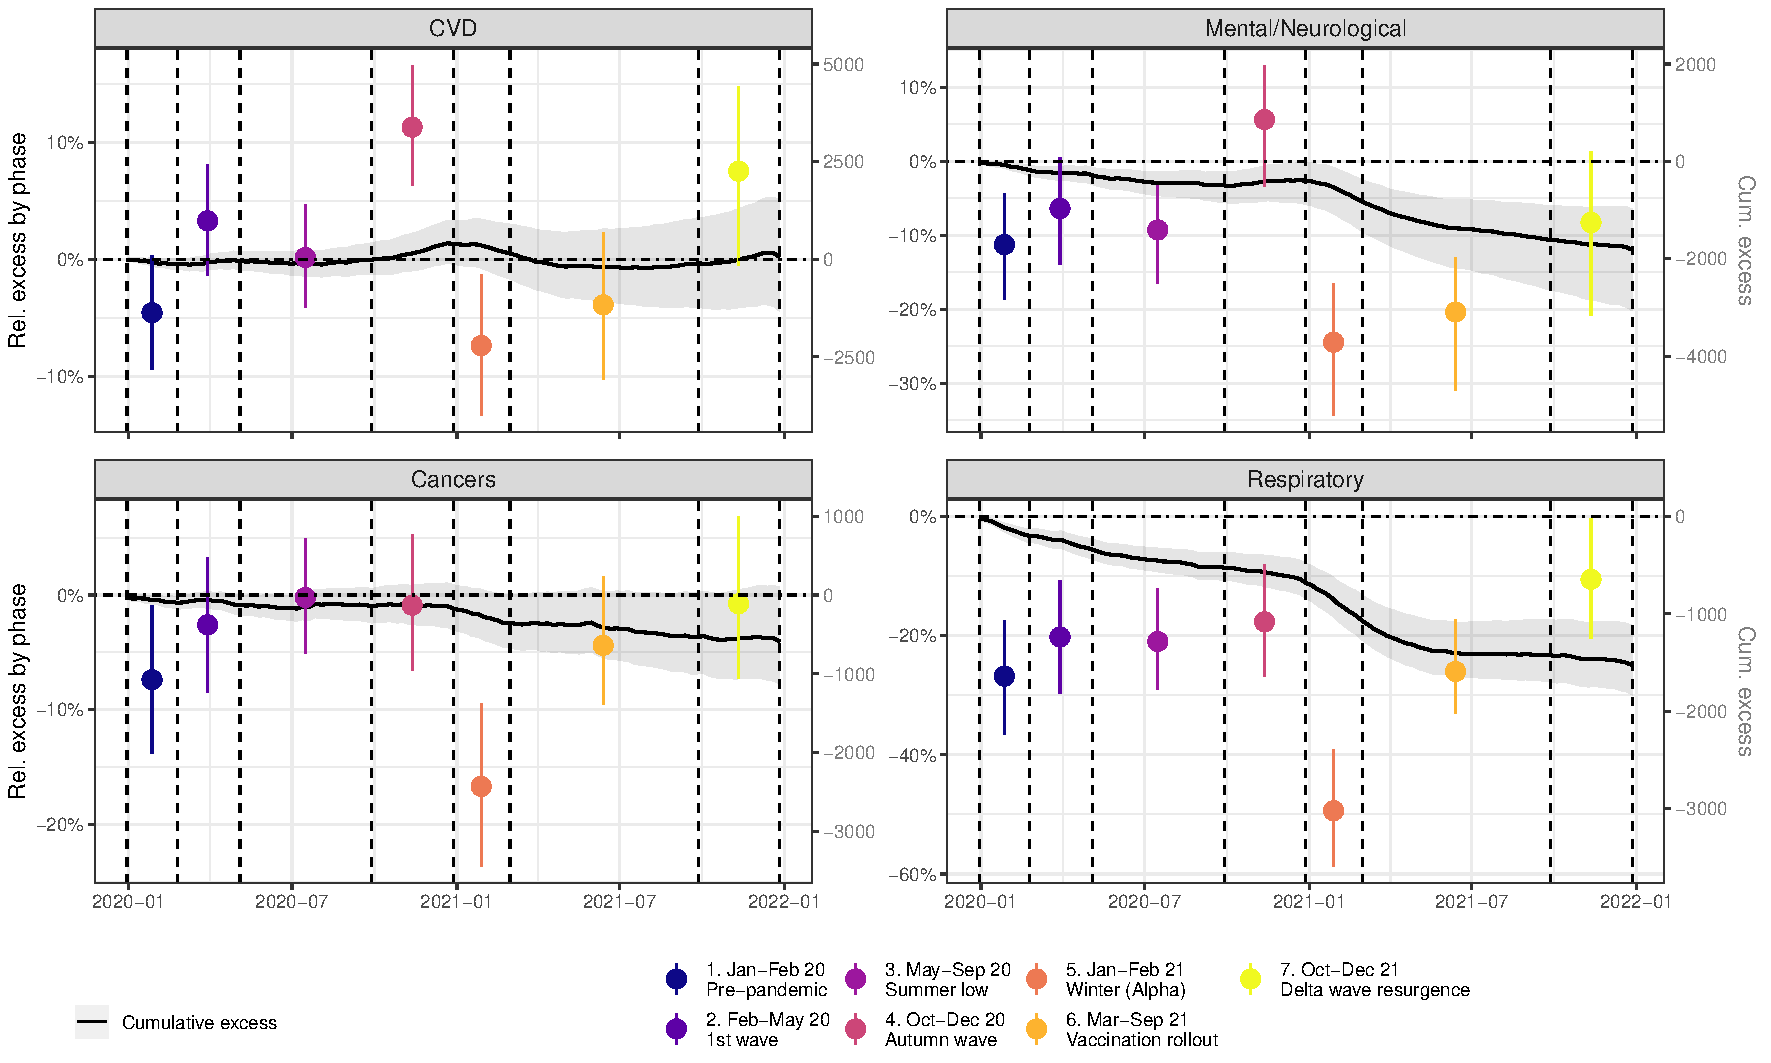
\includegraphics[width=\linewidth,height=0.72\textheight,keepaspectratio]{fig3_v2.pdf}\\[0.2em]
      \figcaption{\textbf{Figure 3. Cause-specific excess mortality by phase in 80+.}
        Black lines (with gray 95\% CrI) show cumulative excess mortality in
        2020--21. Colored points and bars indicate phase-specific relative excess
        mortality (95\% CrI).}
    \end{column}
  \end{columns}
\end{frame}

\begin{frame}{Cancer exploration}
  \begin{itemize}\compresslist
    \item The deficit in cancer deaths was investigated using
          \textbf{multiple-cause-of-death} data.
    \item Total deaths \emph{with} cancer did not decline in January--February 2021;
          slight increase in the 65--79 age group, larger in 80+.
    \item The largest increase was observed for \textbf{high-survival cancers},
          particularly in the 80+ age group.
    \item Interpretation: cancer patients died \emph{from} COVID-19 rather than
          \emph{from} cancer, rather than a genuine drop in cancer deaths.
  \end{itemize}
\end{frame}

%%% Results 4 %%%%%%%%%%%%%%%%%%%%%%%%%%%%%%%%%%%%%%%%%%%%%%%%%%%%%%%%%%%%%%%%%
\begin{frame}{Correlation between excess mortalities}
  \begin{columns}[t]
    \begin{column}{0.45\linewidth}
      \begin{itemize}\compresslist
        \item Strong positive partial correlations (up to $\sim 0.5$) between
              COVID-19 excess mortality and excess deaths from CVD and
              mental/neurological diseases.
        \item Similar positive correlations with other respiratory diseases.
        \item Correlations peak at lags of 1--3 weeks: COVID-19 excess deaths
              occurred slightly after CVD and mental/neurological deaths.
        \item Cancer shows weak or negative correlations with COVID-19 mortality.
      \end{itemize}
    \end{column}
    \begin{column}{0.53\linewidth}
      \centering
      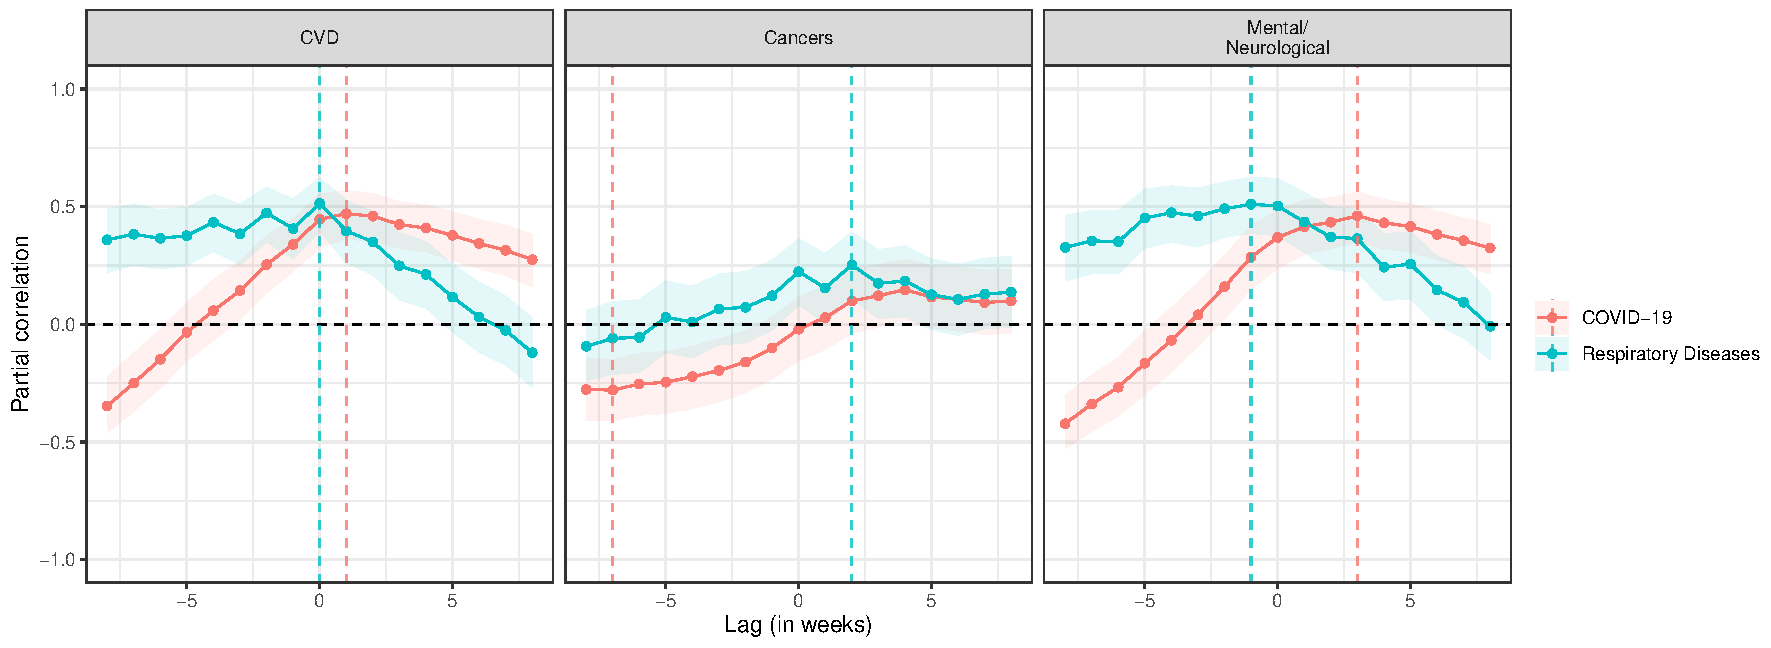
\includegraphics[width=\linewidth,height=0.72\textheight,keepaspectratio]{fig4_v2.pdf}\\[0.2em]
      \figcaption{\textbf{Figure 4.} Partial correlation between excess mortality
        due to either COVID-19 (red) or other respiratory diseases (blue) and
        excess mortality due to CVD, cancers or mental/neurological diseases in 80+.}
    \end{column}
  \end{columns}
\end{frame}

%%% Mechanisms %%%%%%%%%%%%%%%%%%%%%%%%%%%%%%%%%%%%%%%%%%%%%%%%%%%%%%%%%%%%%%%%
\begin{frame}{Mechanisms of mortality disruption}
  \centering
  {\scriptsize
  \begin{tabular}{p{2.4cm} p{4.2cm} p{5.2cm}}
    \toprule
    \textbf{Mechanism} & \textbf{Explanation} & \textbf{Examples} \\
    \midrule
    \raggedright Under-ascertainment of COVID-19 deaths &
      COVID-19 infections not identified at the time of death inflated mortality
      attributed to other causes. &
      CVD excess during autumn 2020 aligned with COVID-19 mortality. \\
    \midrule
    \raggedright Delayed SARS-CoV-2 effects &
      Post-infection complications increased risks of death weeks to months after
      infection. &
      Low evidence for Switzerland. \\
    \midrule
    \raggedright Mortality displacement &
      Early deaths among frail individuals reduced deaths expected later, creating
      mortality deficits. &
      Deficits in dementia and CVD deaths following the autumn 2020 wave;
      cancer patients dying from COVID-19 instead of cancer. \\
    \midrule
    \raggedright Pandemic response (NPIs) &
      Control measures reduced circulation of respiratory pathogens and affected
      related causes. &
      Large decrease in non-COVID respiratory mortality; lower winter mortality
      for dependent causes in older adults. \\
    \bottomrule
  \end{tabular}}\\[0.4em]
  \figcaption{\textbf{Table 1.} Potential mechanisms driving mortality disruptions
    during the COVID-19 pandemic.}
\end{frame}

%%% Conclusions %%%%%%%%%%%%%%%%%%%%%%%%%%%%%%%%%%%%%%%%%%%%%%%%%%%%%%%%%%%%%%%
\begin{frame}{Conclusions}
  \begin{itemize}\compresslist
    \item A Bayesian multivariate model jointly estimates cause-specific excess
          mortality and the dependencies between causes.
    \item Excluding COVID-19 deaths, mortality in Switzerland was
          \textbf{lower than expected} in 2020--21.
    \item Excesses and deficits are strongly structured across causes and in time:
          CVD and mental/neurological excesses track COVID-19 waves and are
          followed by deficits.
    \item Four mechanisms --- under-ascertainment, delayed effects, mortality
          displacement and the pandemic response --- jointly explain the observed
          disruptions.
  \end{itemize}
\end{frame}

\begin{frame}[plain]
  \centering
  \vfill
  {\Large\bfseries\color{headerfontcol} Thank you}\\[1em]
  {\small anthony.hauser@unisante.ch}
  \vfill
\end{frame}

\end{document}
